\documentclass[12pt,a4paper,oneside]{article}
\usepackage[colorlinks=true]{hyperref}
\usepackage[utf8]{inputenc}
\usepackage[czech]{babel}
\usepackage{graphicx}
\usepackage{pdfpages}
\usepackage{listings}
\textwidth 16cm \textheight 25cm
\topmargin -1.3cm 
\oddsidemargin 0cm
\pagestyle{empty}
\begin{document}
\title{Emulátor digitálního syntetyzéru od DG8SAQ}
\author{Jakub Kákona, kaklik@mlab.cz}
\maketitle

\thispagestyle{empty}
\begin{abstract}
Vzhledem k tomu, že je potřebné modul CLKGEN01B nějakým způsobem přelaďovat, je vhodné jej připojit například k počítači. Tento článek popisuje způsob, jak ovládat čip Si570 pomocí sběrnice USB. 
\end{abstract}

\begin{figure} [htbp]
\begin{center}
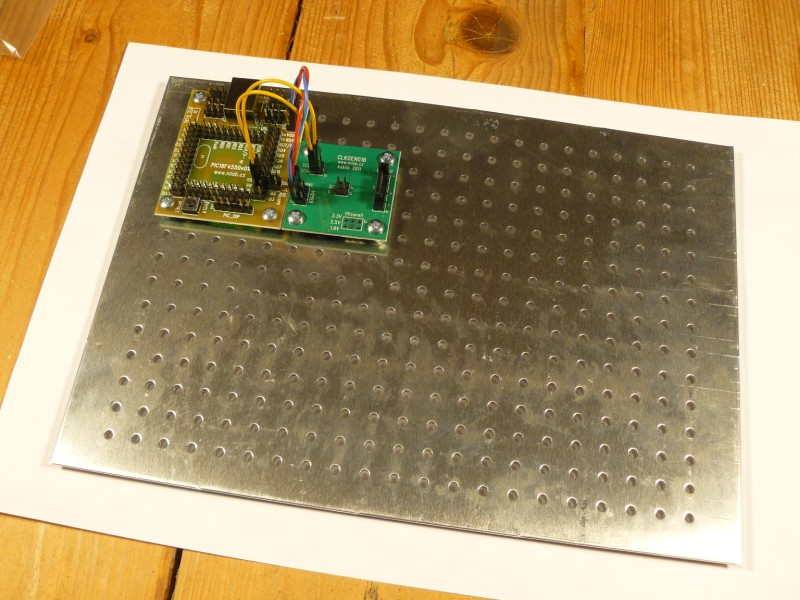
\includegraphics [width=80mm] {DG8SAQ_emulator_Big.jpg} 
\end{center}
\end{figure}

\tableofcontents

\section{Technické parametry}
\begin{table}[htbp]
\begin{center}
\begin{tabular}{|c|c|p{4.7cm}|}
\hline
Parametr & Hodnota & Poznámka \\
\hline
Napájecí napětí POWER  & max 5V &  Napájení z USB\\ 
\hline
Frekvenční rozsah  & 10 - 1500 MHz & Záleží na konkrétním typu čipu Si5XX, obvykle 10-810MHz \\ 
\hline
Fázový jitter  & $<$ 0,3ps & Pro obvody řady Si570 z diferenciálním výstupem\\ 
\hline
\end{tabular}
\end{center}
\end{table}

\section{Popis konstrukce}
Zařízení vychází z velmi rozšířené metody ovládání čipu Si570 pomocí ATtiny, tak jak byla navržena v \cite{Si570board}. Tento postup funguje, ale díky nekompatibilním napěťovým úrovním na USB a na ATtiny, může způsobovat nežádoucí chování. Navíc v některých moderních implementacích USB 3.0 může být jeho použití rizikové pro rozhraní v počítači. Zde je proto popsán technicky mnohem čistší způsob vyhovující standardu USB při zachování všech funkcí původní konstrukce.
Navíc je zde i korektně bezodrazově ošetřen vysokofrekvenční výstup z čipu Si570. 

V nových zařízeních MLAB jako je například stanice RMDS02 je však tento způsob ovládání modulu nahrazen kombinací modulu USBI2C \cite{USBI2C} s knihovnou pymlab\cite{pymlab}. Tento způsob ovládání odstraňuje některé technické problémy vycházející z principu ovládání Si570 přes PIC. (dochází nejčastěji ke ztrátě kmitočtové kalibrace syntezátoru). Při přímém ovládání obvodu Si570 přes I2C tyto komplikace nevznikají. 

\subsection{Zapojení}
Zapojení spočívá pouze v propojení modulu PIC18F4550v01A s modulem CLKGEN01B. Toto je realizováno jedním napájecím kablíkem, který propojuje napájení modulu připojeného na USB s 5V napájením CLKGEN01B (Modul si nižší napájecí napětí stabiluzuje sám). V zapojení jsou ještě dva datové kablíky, které přímo propojují I2C sběrnici.
Na modulu PIC18F4550v01A je jako napájení jumperem zvoleno USB. Použitý krystal je 20 MHz, což vyžaduje v modulu osazené u oscilátoru kondenzátory s kapacitou 12pF.



\subsection{Odrušení}

Odrušení je třeba provádět zvláště pečlivě, pracujeme-li v prostředí, kde by mohlo vadit elektromagnetické vyzařování, jako jsou například radioastronomická pracoviště. Nejkritičtějším místem je v tomto případě připojení počítače, který je často sám o sobě silným zdrojem rušení. USB kabel je tedy vhodné volit dostatečně stíněný a nejlépe s odrušovacími ferity na obou koncích. Počítač by sám o sobě měl do USB vnášet co nejmenší množství šumu, proto je dobré použít místo notebooku spíše stolní počítač s kvalitním zdrojem a kovovou bednou. Samozřejmost je mít moduly přišroubované na dostatečně vodivé podložce tedy nejlépe ALBASE.  

\section{Nastavení testování}
Při připojení k napájení generuje CLKGEN01B frekvenci nastavenou při výrobě v Silicon Labs. V případě modulů MLAB je to 10~MHz z důvodu využitelnosti jako standardní laboratorní normál.  Pro možnost ladění je potřeba do PIC18F4550 nahrát firmware, který naleznete na \cite{pic_firmware}. Při úspěšném nahrání firmwaru programátorem například PICprogUSB02A, se sestava připojením k počítači ohlásí jako nové USB zařízení a bude vyžadovat driver. Ten lze ten je stejný jako pro původní konstrukci a lze jej nalézt v odkazu\cite{CFGSR}.

\noindent Firmware do modulu nahrajeme skriptem, který se nachází ve složce SW. Skript spustíme přes příkazový řádek:

\begin{lstlisting}[language=bash]
svnMLAB/Modules/Clock/CLKGEN01B/SW$ ./flash.sh
Program Succeeded.
PICkit 2 Verify Report
16-1-2016, 18:16:56
Device Type: PIC18F4550

Verify Succeeded.

Operation Succeeded
\end{lstlisting}


\section{Programové vybavení}
Vzhledem k tomu, že výsledek je plně kompatibilní s  konstrukcí dg8saq lze k ladění generátoru použít naprostou většinu programů pro SDR a nebo pouze pro nastavení frekvence například USBSynth \cite{USB_Synth}, či CFGSR \cite{CFGSR}, které je z těchto nástrojů nejmodernější.

\begin{thebibliography}{99}
\bibitem{Si570board}{Původní konstrukce Si570 Board } 
\href{http://wb6dhw.com/inactive.html}{http://wb6dhw.com/inactive.html}

\bibitem{DG8SAQemulator}{PIC emulátor USB syntezátoru od DG8SAQ} 
\href{http://www.qrpradio.org/pub/softrocks/manuals/Softrock Group Files 210109/21 9V1AL/02 UBW Emulator/README.txt}{http://www.qrpradio.org/pub/softrocks/manuals/Softrock Group Files 210109/21 9V1AL/02 UBW Emulator/README.txt}

\bibitem{CFGSR}{CFGSR} 
\href{http://pe0fko.nl/CFGSR/}{http://pe0fko.nl/CFGSR/}

\bibitem{USB_Synth}{USB Synth}
\href{ http://www.mydarc.de/dg8saq/hidden/USB\_Synth3.zip}{http://www.mydarc.de/dg8saq/hidden/USB\_Synth3.zip}

\bibitem{USBI2C}{USBI2C01A}
\href{http://wiki.mlab.cz/doku.php?id=cs:usbi2c}{http://wiki.mlab.cz/doku.php?id=cs:usbi2c}

\bibitem{pymlab}{pymlab}
\href{http://wiki.mlab.cz/doku.php?id=cs:pymlab}{http://wiki.mlab.cz/doku.php?id=cs:pymlab}

\bibitem{pic_firmware}{PIC firmware}
\href{http://www.mlab.cz/Modules/Clock/CLKGEN01B/SW/DG8SAQ\%20synthesiser\_Emulator/firmware.hex}{http://www.mlab.cz/Modules/Clock/CLKGEN01B/SW/DG8SAQ\%20synthesiser\_Emulator/firmware.hex}


\end{thebibliography}
\end{document}